\documentclass{beamer}
\usepackage[utf8]{inputenc}
\usepackage[utf8]{vietnam}
\usetheme{AnnArbor}
\usepackage{letltxmacro}
\usepackage[english]{babel}

\title{Mutilobjective Evolutionary Optimization}
\author{Taskoverflow}
\date{December 2018}

\begin{document}

\begin{frame}
    \titlepage
\end{frame}
\section[Outline]{}
\begin{frame}   
    \tableofcontents
\end{frame}
\section{INTRODUCTION}
\begin{frame}{INTRODUTION}
    \begin{block}{Point 1}
        Thế nào là bài toán tối ưu đa mục tiêu?
    \end{block}
\end{frame}
\begin{frame}{Bài toán tối ưu đa mục tiêu trong thực tế}
    \begin{block}{Mục tiêu 1}
        Quãng đường
    \end{block}
    \begin{block}{Mục tiêu 2}
        Thời gian
    \end{block}
\end{frame}
\begin{frame}{Bài toán tối ưu đa mục tiêu trong thực tế}
    \begin{itemize}
        \item <1-> Với nhiêu liệu có trước, công sinh A sinh ra là cố định.
        \item <2-> Thời gian t giảm khi vận tốc v tăng
        \item <3-> Vận tốc v tăng thì lực cản tăng, công hao phí tăng 
        \item <4-> Công hao phí tăng, quãng đường có thể đi được giảm
    \end{itemize}
\end{frame}
\begin{frame}{Các định nghĩa cơ bản}
    \begin{block}{Không gian nghiệm}
        Với các điều kiện rằng buộc của $x$ sẽ xác định một không gian $\Omega \subset R^{n}$
    \end{block}
    \pause
    \begin{block}{Hàm mục tiêu}
             $y = f(x)= (f_{1}(x),...,f_{m}(x))$
             \\$ x \in \Omega $
    \end{block}
    \pause
    \begin{block}{Không gian mục tiêu}
        $f : \Omega \to \Theta  \subset R^{m}$ xác định không gian mục tiêu $\Theta$
    \end{block}
\end{frame}
\begin{frame}{Hình ảnh minh họa}
    \begin{figure}
    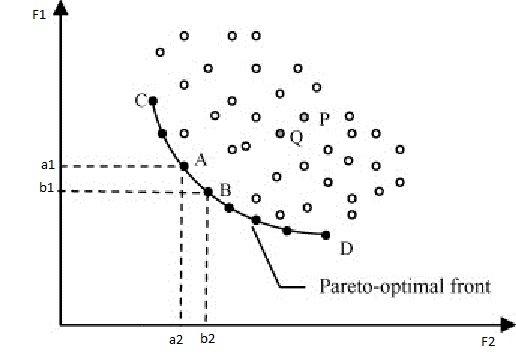
\includegraphics[scale = 0.6]{paretofront.jpg}
    \caption{Nguồn: Science Direct}
    \end{figure}
\end{frame}
\begin{frame}{Các định nghĩa cơ bản}
    \begin{columns}
    \column{0.6\textwidth}
    \begin{figure}
        \centering
        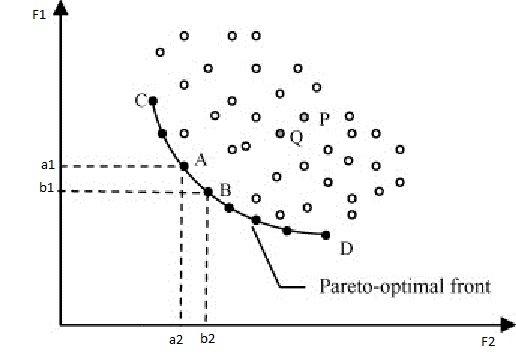
\includegraphics[scale = 0.5]{paretofront.jpg}
        \caption{Hình ảnh minh họa}
        \label{fig:my_label}
    \end{figure}
    \column{0.4\textwidth}
    \pause
     Cho 2 nghiệm $x,y \in \Omega $, $x$ trội hơn $y$ nếu như $\forall i \in {1,2,...,m}, f_{i}(x) \leq f_{i}(y)$ và $ \exists j \in {1,2,...,m}, f_{j}(x) < f_{j}(y)$. 
    \end{columns}
\end{frame}
\begin{frame}{Các định nghĩa cơ bản}
    \begin{columns}
    \column{0.6\textwidth}
    \begin{figure}
        \centering
        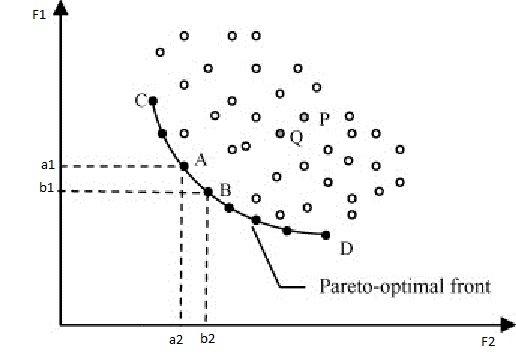
\includegraphics[scale = 0.5]{paretofront.jpg}
        \caption{Hình ảnh minh họa}
        \label{fig:my_label}
    \end{figure}
    \column{0.4\textwidth}
     Một nghiệm $x^{*} \in \Omega$ là nghiệm tối ưu Pareto nếu không tồn tại $x \in \Omega$ trội hơn nó
    \end{columns}
\end{frame}
\begin{frame}{Các định nghĩa cơ bản}
    \begin{columns}
    \column{0.6\textwidth}
    \begin{figure}
        \centering
        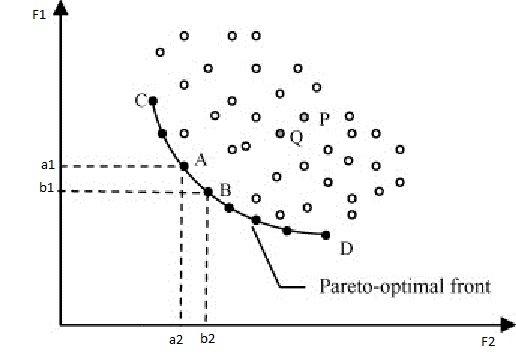
\includegraphics[scale = 0.5]{paretofront.jpg}
        \caption{Hình ảnh minh họa}
        \label{fig:my_label}
    \end{figure}
    \column{0.4\textwidth}
     Tập hợp nghiệm tối ưu Pareto được gọi là tập Pareto.
    \end{columns}
\end{frame}
\begin{frame}{Các định nghĩa cơ bản}
    \begin{columns}
    \column{0.6\textwidth}
    \begin{figure}
        \centering
        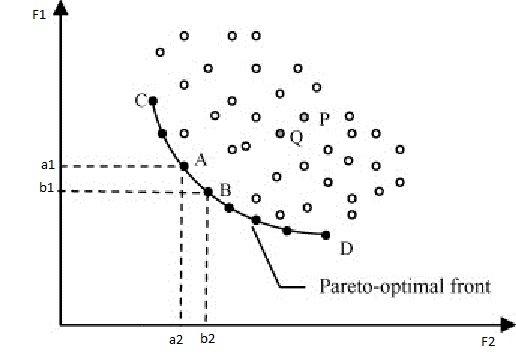
\includegraphics[scale = 0.5]{paretofront.jpg}
        \caption{Hình ảnh minh họa}
        \label{fig:my_label}
    \end{figure}
    \column{0.4\textwidth}
    Các vector mục tiêu tương ứng của tập Pareto được gọi là Biên Parato(PF).
    \end{columns}
\end{frame}
\begin{frame}{Mục tiêu tối ưu}
    Mục tiêu tối ưu là đạt được một tập xấp xỉ S với tập biên Pareto thỏa mãn:
    \pause
    \begin{block}{Độ hội tụ}
        Mọi nghiệm thuộc S là gần nhất có thể với P.
        \end{block}
    \pause
    \begin{block}{Độ đa dạng}
    Mọi nghiệm thuộc S phân bố đa dạng trên không gian mục tiêu
    \end{block}
\end{frame}
\begin{frame}{Hình ảnh minh họa}
    \begin{figure}
    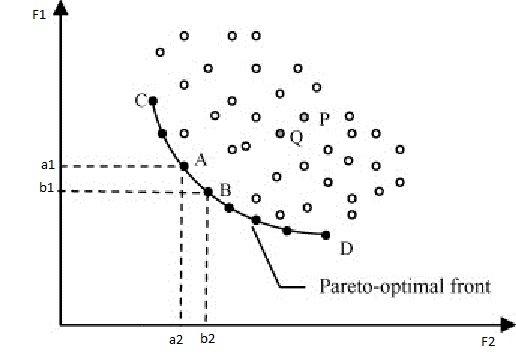
\includegraphics[scale = 0.6]{paretofront.jpg}
    \caption{Nguồn: Science Direct}
    \end{figure}
\end{frame}


%--------------------------------------------------------------------------------


\section{Các bài toán nhiều mục tiêu}

\begin{frame}{MANY OBJECTIVE PROBLEM (MoAPs)}
    \begin{itemize}
        \item <1-> Không có định nghĩa chung cho MaOPs
        \item <2-> Động lực chính đằng sau MaOPs là làm nổi bật những thách thức đặt ra bởi một số lượng lớn các mục tiêu cho các thuật toán tiến hóa đa mục tiêu (MOEAs) hiện tại
        \item <3-> Hiện tại ta có thể định nghĩa MaOPs là các bài toán đa mục tiêu MOPs với $m \geq 4$
    \end{itemize}
\end{frame}

\begin{frame}{KHÓ KHĂN}
{Các khó khăn trong quá trình giải quyết các bài toán nhiều mục tiêu (Many Objectives)}
    \begin{itemize}
        \item <1-> Phần lớn các cá thể là không trội, không thể sắp xếp được
        \item <2-> Tính toán độ đa dạng thuật toán trở nên khó khăn
        \item <3-> Quá trình tái tổ hợp có thể không hiệu quả
        \item <4-> Việc thể hiện sự trade-off surface khó khăn
        \item <5-> Tốn thời gian để so sánh hiệu suất giữa các thuật toán với nhau (Performance metrics)
        \item <6-> Rất khó để biểu diễn lời giải một cách trực quan
    \end{itemize}
\end{frame}
\begin{frame}{Hai ý tưởng cho Many Objective EMO}
    \begin{block}{1.}
        Sử dụng nguyên tắc trội đặc biệt:$\varepsilon$-domination, mating restriction scheme or special recombination scheme (SBX với large distribution index,…)
    \end{block}
    \pause
    \begin{block}{2.}
        Sử dụng nền tảng của các nghiên cứu đa mục tiêu trước
    \end{block}
\end{frame}
\end{document}
